%%%%%%%%%%%%%%%%%%%%%%%%%%%%%%%%%%%%%%%%%%%%%%%%%%%%%%%%%%%%%%%%%%%%%%%%%%%%%%%
%% Agentic JWST strong-lens search — research paper draft.
%%
%% Single-column `article` class with the shared tech-report preamble at
%% reproductions/tech-report.sty. Builds with vanilla TeX Live (>= 2022).
%% An AASTeX port for journal submission is planned as a sibling document;
%% the preamble already uses only AASTeX-compatible astronomy macros.
%%%%%%%%%%%%%%%%%%%%%%%%%%%%%%%%%%%%%%%%%%%%%%%%%%%%%%%%%%%%%%%%%%%%%%%%%%%%%%%
\documentclass[11pt,letterpaper]{article}
\usepackage{../../tech-report}
\usepackage{longtable}

% Paper-specific macros
\newcommand{\thetaE}{\ensuremath{\theta_{\mathrm{E}}}}
\newcommand{\Msun}{\ensuremath{M_\odot}}
\newcommand{\cc}{\textsc{Claude Code}}
\newcommand{\numtargets}{5{,}391}
\newcommand{\numinspected}{5{,}308}
\newcommand{\numflagged}{2{,}024}

\title{An Agentic AI Search for Galaxy-Scale Strong Gravitational Lenses\\
       in the Public JWST NIRCam Archive}
\author{Gregory D.~Benson$^{1}$ \and Xiaosheng Huang$^{2,3}$ \and Nathan Kvinnesland$^{1}$}
\date{August 2026 \\[2pt]
  {\small $^{1}$Department of Computer Science, University of San Francisco\\
  $^{2}$Department of Physics \& Astronomy, University of San Francisco\\
  $^{3}$Lawrence Berkeley National Laboratory}\\[4pt]
  \texttt{DRAFT — prepared for arXiv submission}}
\addbibresource{references.bib}

\begin{document}

\maketitle
\subtitle{Research Paper Draft}

\begin{abstract}
We report the first archive-wide search for galaxy-scale strong gravitational
lenses conducted end-to-end by a general-purpose agentic AI. Using \cc{}
(v2.1.224, model \texttt{claude-opus-5}), initiated by a single natural-language
prompt, the agent designed and live-verified its own search pipeline, wrote and
ran all code, and then acted as its own visual inspector, adversarial verifier,
and literature auditor. From a census of 6{,}848 public JWST/NIRCam
calibration-level-3 observations ($t_{\rm exp}>1000$\,s; 916 distinct fields;
4.48\,deg$^2$ of unique sky), the agent selected the complete population of
\numtargets{} Legacy Surveys elliptical galaxies with $r<21$, streamed
$10''$ cutouts directly from the MAST S3 archive, and visually inspected
\numinspected{} rendered cutouts (100\%) with vision subagents, including 31
blind-injected COWLS lenses as positive controls. A three-persona adversarial
verification stage (instrument-artifact, morphology, and lensing-geometry
refuters) reduced \numflagged{} flagged cutouts to a ranked top-100, with blind
Einstein-radius estimates and an independent literature crossmatch. The search
re-discovered published lenses without prior knowledge --- rank~1 is the
double-source-plane lens SL2S\,J02176-0513 --- while an independent audit finds
66 of the top 100 have no prior identification, including two grade-A
galaxy-scale candidates and a group-scale system whose deflector is the
brightest cluster galaxy of WH\,J135810.5-105636, with blind
$\thetaE=3.6''\pm0.4''$ implying $M(<22\,\mathrm{kpc})\approx3\times10^{12}\,\Msun$.
The campaign consumed $\sim$76.5M billable tokens across 1{,}281 subagents on
a consumer subscription; the discovery pipeline itself ran in $\sim$40 hours
of wall-clock, roughly half of it waiting out usage-limit windows. The complete 2.2\,GB corpus of agent
transcripts is preserved, and we analyze it to characterize \emph{how} the
agent reasons about lensing evidence: a recall-biased screening pass that never
asserted a confident false detection, refutation by named astrophysical
mechanisms, and unprompted escalation from visual inspection to quantitative
image analysis. We discuss completeness limits (48\% recovery of injected
controls; 54\% of 239 catalogued lenses on inspected cutouts), calibration
weaknesses, and the human-AI alignment loop this workflow enables.
\end{abstract}

\tableofcontents

\bigskip

% =============================================================================
\section{Introduction}\label{sec:intro}
% =============================================================================

Galaxy-scale strong gravitational lenses are precision instruments: they weigh
galaxy dark-matter halos, magnify high-redshift sources, and, with
time-variable sources, constrain $H_0$. They are also rare, of order one per
$\sim$$10^4$ massive ellipticals, so every generation of lens discovery has
been an exercise in scaling human judgement. Visual searches of HST fields
gave way to arc-finders, then to convolutional neural networks applied to
wide-field surveys \citep{petrillo2017finding, jacobs2019extended,
huang2020finding, huang2021discovering, storfer2024new, inchausti2025strong},
to systematic benchmarking \citep{metcalf2019strong}, and to crowdsourcing
\citep{marshall2016spacewarps, garvin2022hubble}. In the JWST era, the
COSMOS-Web Lens Survey (COWLS) combined expert visual inspection over a single
contiguous mosaic to find $>$400 candidates in 0.54\,deg$^2$
\citep{nightingale2025cowls1, mahler2025cowls2}.

The public JWST archive as a whole, however, resists all of these approaches.
It is not a survey: it is thousands of heterogeneous pointings in dozens of
filter combinations, depths, and pipeline versions
\citep{gardner2023jwst, rieke2023nircam}. No training set exists that matches
its selection function, so supervised CNNs cannot be applied off the shelf;
and its footprint is too scattered and too deep for a volunteer campaign to
cover quickly. Meanwhile, large multimodal language models have reached the
point where a single system can write and execute code against live
astronomical services, read images, argue about morphology in astrophysical
vocabulary, and search the literature --- the full skill set of a lens-search
team, if not yet its judgement.

This paper reports what happens when that experiment is actually run. We gave
\cc{} \citep{anthropic2025claudecode}, a general-purpose agentic AI operating a
terminal on a consumer laptop, the following prompt (verbatim; see
Appendix~\ref{app:prompts}):

\begin{quote}\itshape
``We want to try a one-shot galaxy scale strong lens search in the JWST
archive. Limit this search to observations with exposure times greater than
1000 seconds that are publically available. Make cutouts that are 10 arc
seconds wide centered on a galaxy that is brighter than 21st magnitude. Look
at every cutout and determine whether it contains a strong lens. [\ldots] For
now, I would like to see the top 100 candidates.''
\end{quote}

Everything downstream of that prompt --- the archive census, the deflector
catalog queries, the streaming cutout service, the decision to inject blind
positive controls, the inspection prompts, the adversarial verification
design, the ranking, and the literature crossmatch --- was designed and
executed by the agent, with the human operator supervising, approving the
plan, and re-launching stages after usage-limit interruptions. To our
knowledge this is the first strong-lens discovery campaign, and among the
first astronomical discovery campaigns of any kind, run end-to-end by an
agentic AI on a public archive.

Our contributions are:
\begin{enumerate}
  \item \textbf{A complete archive-scale search} of public JWST NIRCam imaging
    around \numtargets{} bright elliptical deflectors --- the complete
    $r<21$ population in the covered footprint, not a sample --- producing a
    ranked top-100 candidate list with per-candidate evidence text, blind
    Einstein-radius estimates, deflector redshifts, and prior-identification
    status (Appendix~\ref{app:top100}).
  \item \textbf{Blind validation inside the run}: 31 COWLS lenses
    \citep{nightingale2025cowls1} injected with randomized identifiers,
    plus an after-the-fact completeness measurement against 239 catalogued
    lenses that happen to fall on inspected cutouts.
  \item \textbf{An independently audited novelty assessment}: 10 of the top
    100 are published lenses (led by the double-source-plane system
    SL2S\,J02176-0513 at rank 1), 24 sit in known cluster strong-lensing
    fields, and 66 carry no prior identification.
  \item \textbf{New candidates}, including two clean grade-A galaxy-scale
    systems and a group-scale arc system around the brightest cluster galaxy
    of the \citet{wen2024catalog} cluster WH\,J135810.5-105636
    (Section~\ref{sec:gem}).
  \item \textbf{A reasoning corpus and its analysis}: 1{,}281 per-agent
    transcripts (2.2\,GB) recording every image the system looked at, every
    tool call, and every verdict rationale. Section~\ref{sec:reasoning} mines
    this corpus to describe how the agent actually identifies lenses ---
    including behaviors we did not prompt for.
\end{enumerate}

Section~\ref{sec:data} describes the archive census and target selection;
Section~\ref{sec:pipeline} the agentic pipeline; Section~\ref{sec:results} the
candidate list, control recovery, and audit; Section~\ref{sec:reasoning} the
transcript analysis; Section~\ref{sec:discussion} compares this modality with
CNN and citizen-science searches and lays out the human-alignment loop;
Section~\ref{sec:conclusions} concludes. Throughout we use the
\citet{planck2020params} cosmology.

% =============================================================================
\section{Data}\label{sec:data}
% =============================================================================

\subsection{JWST archive census}\label{sec:census}

A single MAST \code{astroquery} census returned all public JWST/NIRCam
calibration-level-3 \code{i2d} mosaics with $t_{\rm exp}>1000$\,s: 6{,}848
observations. Footprint-overlap clustering (union-find on the \code{s\_region}
polygons) grouped them into 916 distinct sky fields covering 4.48\,deg$^2$ of
unique sky. No mosaics were downloaded: the agent verified during planning
that the MAST public S3 mirror (\code{stpubdata}) serves uncompressed SCI
extensions that support true HTTP ranged reads via
\code{astropy.io.fits} + \code{fsspec}, so every cutout was streamed as a
$\sim$$10''$ section directly from the cloud. The entire run stayed under
1\,GB of local disk --- a constraint the agent discovered (a nearly full
volume) and designed around.

\subsection{Deflector selection}\label{sec:deflectors}

Deflectors are massive ellipticals from the DESI Legacy Imaging Surveys
\citep{dey2019overview}: DR10 (south) and DR9 (north), queried per field
through the NOIRLab Data Lab TAP service. The selection is
$r_{\rm dered}<21$ with Tractor type \code{DEV}, or \code{SER} with S\'ersic
index $n\geq2.5$; a soft red-sequence cut $r-z>0.4$ (rejections logged, not
silently dropped); \code{BRIGHT}/\code{MEDIUM} maskbit exclusion;
$\code{shape\_r}<8''$; $1''$ deduplication; and a tangent-plane
point-in-polygon test against each observation's actual footprint with a
$6''$ inset. DR11 catalogs were confirmed to not be publicly served (the
viewer exposes DR11 imagery only), so DR10/DR9 were used. A per-field cap of
60 targets (brightest first) preceded a global brightest-first trim. The final
list contains \numtargets{} entries: 5{,}360 archive galaxies --- the complete
selected population in the covered footprint --- plus 31 blind controls
(Section~\ref{sec:controls}).

Each target was assigned its best short-wavelength observation (preference
order F150W, F200W, F115W, F090W, F210M, F150W2; deepest-exposure tiebreak)
and best long-wavelength observation (F277W, F356W, F444W, F410M, F322W2).

\subsection{Cutouts}\label{sec:cutouts}

For each target the agent rendered one JPEG with six panels in two rows: the
full $10''\times10''$ field in (a) a shallow asinh stretch, (b) a deep asinh
stretch, and (c) a two-band color composite (LW resampled onto the SW grid via
WCS); and a central $3.5''$ zoom row showing (d) the deep stretch, (e) the
color composite, and (f) a deflector-subtracted residual computed by radial
profile subtraction. Panels carry a $1''$ scale bar, N/E compass, four yellow
tick marks locating the catalogued galaxy, and corner quadrant labels
(NE/NW/SE/SW). Of \numtargets{} targets, \numinspected{} rendered successfully
and were inspected --- 100\% of renderable targets, with zero malformed
verdicts --- while 83 fell in NIRCam module gaps or had insufficient valid
pixels.

\subsection{Blind positive controls}\label{sec:controls}

The agent's plan --- adopted before any inspection began --- injected 31
known and candidate lenses from the COWLS catalog
\citep{nightingale2025cowls1,mahler2025cowls2} into the target stream with
randomized identifiers, indistinguishable from ordinary targets in the
manifest. The control key was held aside and unblinded only at the reporting
stage. The controls span COWLS ranking codes from unanimous grade-A to
low-confidence candidates, with catalogued Einstein radii up to
$\sim$$2''$.

% =============================================================================
\section{The agentic pipeline}\label{sec:pipeline}
% =============================================================================

\subsection{Agent architecture and provenance}\label{sec:architecture}

The search was run in \cc{} v2.1.224 with the \texttt{claude-opus-5} model
\citep{anthropic2025claudecode, anthropic2026opus} on a consumer subscription
--- these facts, along with per-message token usage and timestamps, are
recorded on every line of the session transcripts, which makes the entire run
auditable after the fact (Section~\ref{sec:reasoning}). The architecture has
three tiers: an interactive \emph{orchestrator} session that talks to the
operator, writes code, and launches work; deterministic \emph{workflow}
scripts that fan work out over parallel subagents with structured-output
schemas; and the \emph{subagents} themselves, each a fresh context that reads
its assignment from a file, works with the full tool set (file reads,
including images, shell, web), and returns validated JSON.

Three sessions comprise the campaign: two short \emph{design} sessions and the
main \emph{discovery} session. The design sessions are notable for what they
did before writing the plan: read-only subagents live-probed every external
interface the plan would depend on --- the S3 ranged-read path, the Data Lab
TAP endpoints and their working ADQL dialect, PyPI wheel availability for the
local Python, catalog-viewer fallbacks, disk headroom, and network
reachability --- so the plan document recorded \emph{verified} facts rather
than assumptions. The resulting \code{PLAN.md} fixed the seven-stage pipeline
of Table~\ref{tab:stages}, the exact selection criteria of
Section~\ref{sec:deflectors}, checkpointing for every stage, and the blind
control injection, and was approved by the operator before execution.

\begin{table}[ht]
\centering
\caption{Pipeline stages with agent counts and billable tokens (input +
output + cache-write), measured from the per-agent transcripts. Wall-clock
spans include usage-limit stalls. The three verification personas each see
every candidate assigned to them; the literature stage runs one agent per
top-100 candidate plus catalog-acquisition agents.}
\label{tab:stages}
\small
\begin{tabular}{@{}llrrrl@{}}
\toprule
Stage & Mechanism & Agents & Killed & Tokens & Wall span (UTC) \\
\midrule
Census, catalogs, cutouts & Python scripts & --- & --- & --- & Aug 8, 00:07--01:47 \\
Plan \& environment probes & design subagents & 4 & 0 & 0.8M & Aug 8, 00:07--00:59 \\
S5 vision inspection & 13 workflows & 537 & 90 & 27.4M & Aug 8, 01:47--21:23 \\
S6 adversarial verification & 12 workflows & 526 & 326 & 22.0M & Aug 8--9 \\
Literature crossmatch & 8 workflows & 192 & 51 & 23.0M & Aug 9--10 \\
Catalog acquisition & 2 workflows & 11 & 0 & 2.1M & Aug 10 \\
Candidate notes & 3 workflows & 11 & 0 & 1.2M & Aug 10 \\
\midrule
Total & 39 workflows & 1{,}281 & 467 & 76.5M & $\sim$3 days \\
\bottomrule
\end{tabular}
\end{table}

\subsection{Stage S5: vision inspection}\label{sec:inspection}

Every rendered cutout was assigned, in deterministic shuffled batches of
$\sim$12--20, to one of 537 vision subagents across 13 workflows. Each agent
was instructed to \code{Read} every image in its batch --- the tool renders
the JPEG into the model's visual context --- and to append one JSON verdict
per cutout: \code{lens\_at\_center} (\code{yes}/\code{likely}/\code{no}),
\code{quadrant\_lens} (\code{none}/NE/NW/SE/SW), an \code{evidence} array,
a \code{center\_galaxy\_type} classification, and a 0--100 confidence.

The inspection prompt (Appendix~\ref{app:prompts}) is a compact field guide:
positive evidence (tangential arcs concave toward the deflector, multiple
images at common radius and color, counter-images, blue-vs-red color
contrast, features surviving in the residual panel) and named false-positive
classes to rule out (spiral arms, collisional rings, edge-on disks, tidal
debris, shells, diffraction spikes, chance alignments, and symmetric
over-subtraction residuals). Critically, it declares the pass's operating
point: \emph{``this is a high-recall first pass \ldots{} the cost of a false
alarm here is low, and the cost of a miss is total.''} Verdict files are
append-only JSONL with resume-on-restart, which mattered:
Section~\ref{sec:cost}.

\subsection{Stage S6: adversarial verification}\label{sec:verification}

All \numflagged{} flagged cutouts (\code{yes} or \code{likely} at center, or
a quadrant flag) were scored, and the top 350 were passed to verification.
Each candidate was re-examined by three independent subagent personas, each
prompted to \emph{refute} the lens claim from a different angle
(Appendix~\ref{app:prompts}):

\begin{itemize}
  \item \textbf{Instrument-artifact specialist}: diffraction spikes,
    snowballs, persistence, mosaic seams, striping, saturation bleed, and
    the symmetric over-/under-subtraction rings of the residual panel;
  \item \textbf{Galaxy-morphology specialist}: spiral arms, collisional and
    resonance rings, shells, tidal tails, mergers, edge-on disks, chance
    alignments;
  \item \textbf{Lensing-geometry specialist}: is the curvature concave toward
    the deflector with its center of curvature at the centroid, tangential
    elongation, counter-image or plausible image multiplicity, a plausible
    \thetaE{} for the deflector's luminosity, and color consistency among
    putative images of one source.
\end{itemize}

Each persona returns \code{pass}/\code{fail}/\code{uncertain} plus a named
alternative explanation. The final grade is the pass count: A $=3$, B $=2$,
C $=1$, D $=0$; flagged candidates outside the verified 350 are grade U. The
ranking that produces the top 100 weights verifier grade above inspector
confidence.

\subsection{Blind \thetaE{} measurement and literature crossmatch}
\label{sec:blindtheta}

Two further workflow families operated on the top 100 only. \emph{Measurement}
agents re-derived arc radii, position angles, counter-image assignments, and a
geometric Einstein-radius estimate (arc radius, or half the image separation)
from the imaging alone, with all published metadata withheld; these are the
blind \thetaE{} values of Table~\ref{tab:top100}. \emph{Literature} agents ---
one per candidate --- converted coordinates, queried SIMBAD, NED, and VizieR,
ran web searches on both coordinate forms, identified the JWST program, and in
several cases fetched and read survey papers (\code{pdftotext} + string
search) to decide between ``published lens,'' ``lens-adjacent field,'' and
``no prior identification.'' A separate catalog-acquisition family assembled
$\sim$195{,}000 catalogued lens and candidate entries (SIMBAD lens types,
COWLS, the DESI-survey lens compilations of
\citealt{huang2020finding,huang2021discovering,storfer2024new,inchausti2025strong},
and others) for uniform crossmatching.

\subsection{Cost, interruptions, and robustness}\label{sec:cost}

Table~\ref{tab:stages} gives the accounting, measured directly from the
per-message usage metadata in the 1{,}281 preserved transcripts: 76.5M
billable tokens (8.5M output), 10{,}853 image reads, 5{,}053 shell commands,
and 2{,}466 web queries. The discovery pipeline itself (inspection +
verification) cost 49.4M tokens --- about 5{,}200 tokens per cutout inspected
and $\sim$21{,}000 per adversarial judgement --- with the literature audit
adding 26.3M more.

The dominant operational failure mode was the subscription's usage limit: 467
of 1{,}281 subagent transcripts (36\%) are stubs killed at launch by the
limit, concentrated in the verification stage (326/526; the first verification
tier lost 78--81\% of its agents). The run's own in-session accounting
attributes $\sim$21\% of tokens to agents killed mid-flight, whose partial
work was discarded. Because every stage checkpointed (append-only verdicts,
skip-if-exists), the orchestrator re-launched only missing work after each
reset: the final verification passes show zero kills and completed the grade
assignments. Total wall-clock from prompt to delivered top-100 was
$\sim$40 hours, roughly half of it waiting out usage-limit windows; the
literature audit ran over the following day.

% =============================================================================
\section{Results}\label{sec:results}
% =============================================================================

\subsection{Verdicts, grades, and demographics}\label{sec:verdicts}

\begin{figure}[ht]
\centering
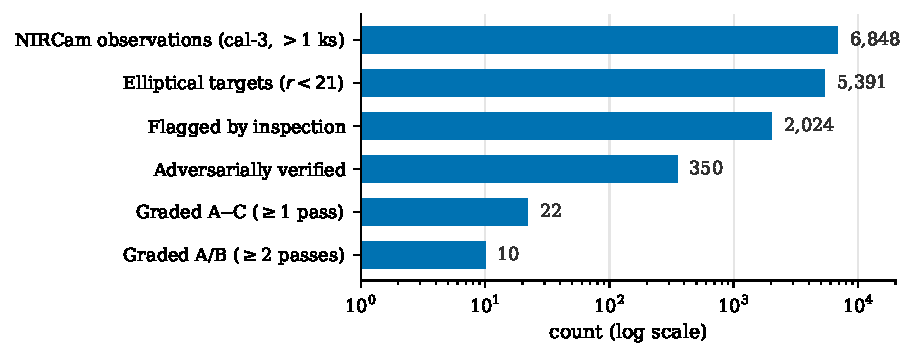
\includegraphics[width=0.78\linewidth]{figures/fig_funnel.pdf}
\caption{The selection funnel, from archive census to verified candidates.
Every step after ``Elliptical targets'' was decided by the agent's own
inspection and verification verdicts.}
\label{fig:funnel}
\end{figure}

Figure~\ref{fig:funnel} summarizes the funnel. Of \numinspected{} inspected
cutouts, the screening pass returned \code{yes} at center for 14,
\code{likely} for 1{,}952, and a quadrant flag for 97; \numflagged{} unique
cutouts entered the flagged pool with evidence text. The 350 verified
candidates resolved into grades A: 5, B: 5, C: 12, D: 328. Central-galaxy
classifications for the remainder are dominated by ellipticals (2{,}084), S0s
(1{,}196), and edge-on disks (434), with mergers (291), spirals (196), stars
(307), and artifacts (48) --- the same confuser classes the verification stage
was designed to kill.

\begin{figure}[ht]
\centering
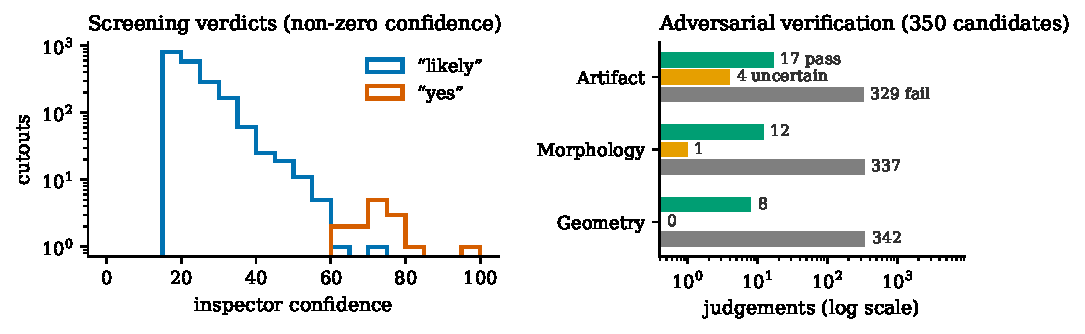
\includegraphics[width=\linewidth]{figures/fig_confidence.pdf}
\caption{\emph{Left:} inspector confidence for non-\code{no} verdicts. The
screening pass behaves as instructed: \code{likely} means ``worth a second
look'' (median confidence 20), and \code{yes} --- median 72, maximum 95 ---
was asserted only 14 times in \numinspected{} cutouts.
\emph{Right:} verification outcomes per persona (log scale); of 350
candidates, each persona passed only 8--17 ($\sim$2--5\%).}
\label{fig:confidence}
\end{figure}

\subsection{Blind control recovery and completeness}\label{sec:completeness}

\begin{figure}[ht]
\centering
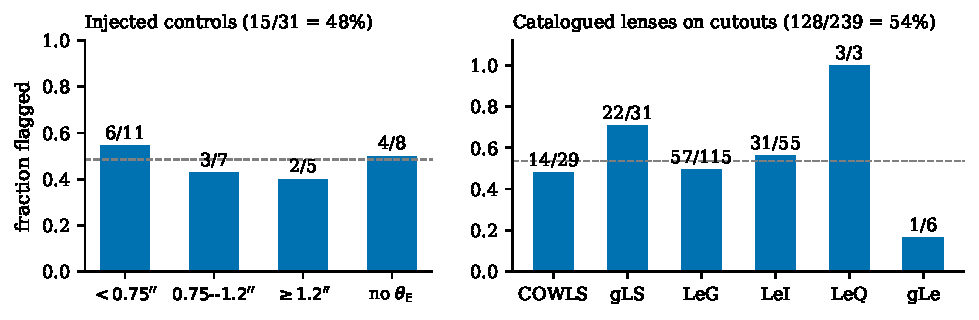
\includegraphics[width=\linewidth]{figures/fig_recovery.pdf}
\caption{\emph{Left:} recovery (flagged by inspection) of the 31
blind-injected COWLS controls, by catalogued Einstein radius.
\emph{Right:} after-the-fact recovery of the 239 catalogued lenses and
candidates that fall on inspected cutouts, by catalog class (SIMBAD lens
types; \code{gLS} = confirmed gravitational lens systems).}
\label{fig:recovery}
\end{figure}

The inspection stage flagged 15 of 31 blind controls (48\%), and 3 of the 5
controls with unanimous COWLS grade-A rankings (Figure~\ref{fig:recovery}).
Recovery shows no strong trend with Einstein radius in this small sample.
No control reached the top 100: recovered controls came back at confidence
15--30 --- inside the \code{likely} shortlist, below the verified tier.

The literature crossmatch enables a second, larger completeness measurement:
239 catalogued lenses and lens candidates happen to fall on inspected cutouts.
The screening pass flagged 128 (54\%) overall, and 22 of 31 (71\%) of the
SIMBAD-confirmed \code{gLS} systems. Of 26 known lenses that entered
verification, the personas passed only 1 --- a $\sim$92\% false-rejection
rate on true lenses. The design conclusion is unambiguous and we state it as
the run's own README does: \emph{a high grade is strong evidence for lensing;
a low grade is not evidence against it.} The verification stage certifies; it
does not grade recall. Completeness at COWLS-like depth is $\sim$50\%, and the
confirmed tier is a floor, not a census.

\subsection{Independent novelty audit}\label{sec:results-xmatch}

The run's own literature verdicts (Table~\ref{tab:top100}, ``Prior ID''
column) report 7 published systems, 90 with no prior identification, and 3
judgement calls. Because novelty claims are the paper's most fragile output,
we re-ran the crossmatch \emph{independently of the discovery session}, in a
separate audited session against 43 catalogs (48{,}004 reference rows local +
NED TAP + SIMBAD otypes + 19 vetted VizieR lens tables), with a dedicated
cluster-lens layer that positional matching alone cannot provide (a cluster's
catalogued coordinate is its center, $1$--$2'$ from any given arc). The audit
finds, out of 100:

\begin{itemize}
  \item \textbf{10 published lenses} (grade A: 2; B: 2; C: 3; U: 3), all
    recovered blind by the pipeline. Rank 1 is SL2S\,J02176-0513
    \citep{cabanac2007sl2s,tu2009sl2s}, the double-source-plane lens: the
    deflector matches at $0.06''$, and the agent's blind
    $\thetaE=1.15''\pm0.20''$ and fold-configuration description match the
    published system (Figure~\ref{fig:rank1}). Rank 4 matches a published
    DESI-survey candidate \citep{inchausti2025strong}; rank 6 a
    citizen-science HST candidate \citep{garvin2022hubble}; others include
    cluster-lensed images in Abell 1689, MACS J0416, and RCS2 J0327 fields.
  \item \textbf{24 in known cluster strong-lensing fields} (e.g., Abell 2537,
    Abell 370, Abell 2744, RELICS and SGAS clusters;
    \citealt{coe2019relics}), where cataloged arcs exist within $\sim$1$'$
    but no specific published arc matches within $5''$. Ten of these sit in
    documented lensing clusters for which no machine-readable arc list could
    be found; those are \emph{unresolved}, not confirmed new.
  \item \textbf{66 with no prior identification} anywhere the audit could
    reach. One caveat inherited by every such verdict: the SLED database is
    login-walled and was never queried.
\end{itemize}

The audit found zero false negatives in the run's own ``known'' labels, but
reclassified 24 of its ``new'' claims as cluster-field --- including one
grade-A and two grade-B systems. The surviving clean grade-A/B unknowns are
ranks 2, 8, and 10, with the qualification that rank 8 lies in the core of the
massive cluster MACS J1105.7$-$1014, whose convergence plausibly boosts a
galaxy-scale deflector. This is the central methodological lesson of the
audit: \emph{for archive searches that revisit famous deep fields, the
dominant re-discovery channel is cluster environments, and a
galaxy-galaxy--style positional crossmatch alone will overstate novelty.}

\subsection{New galaxy-scale candidates}\label{sec:newcands}

\begin{figure}[ht]
\centering
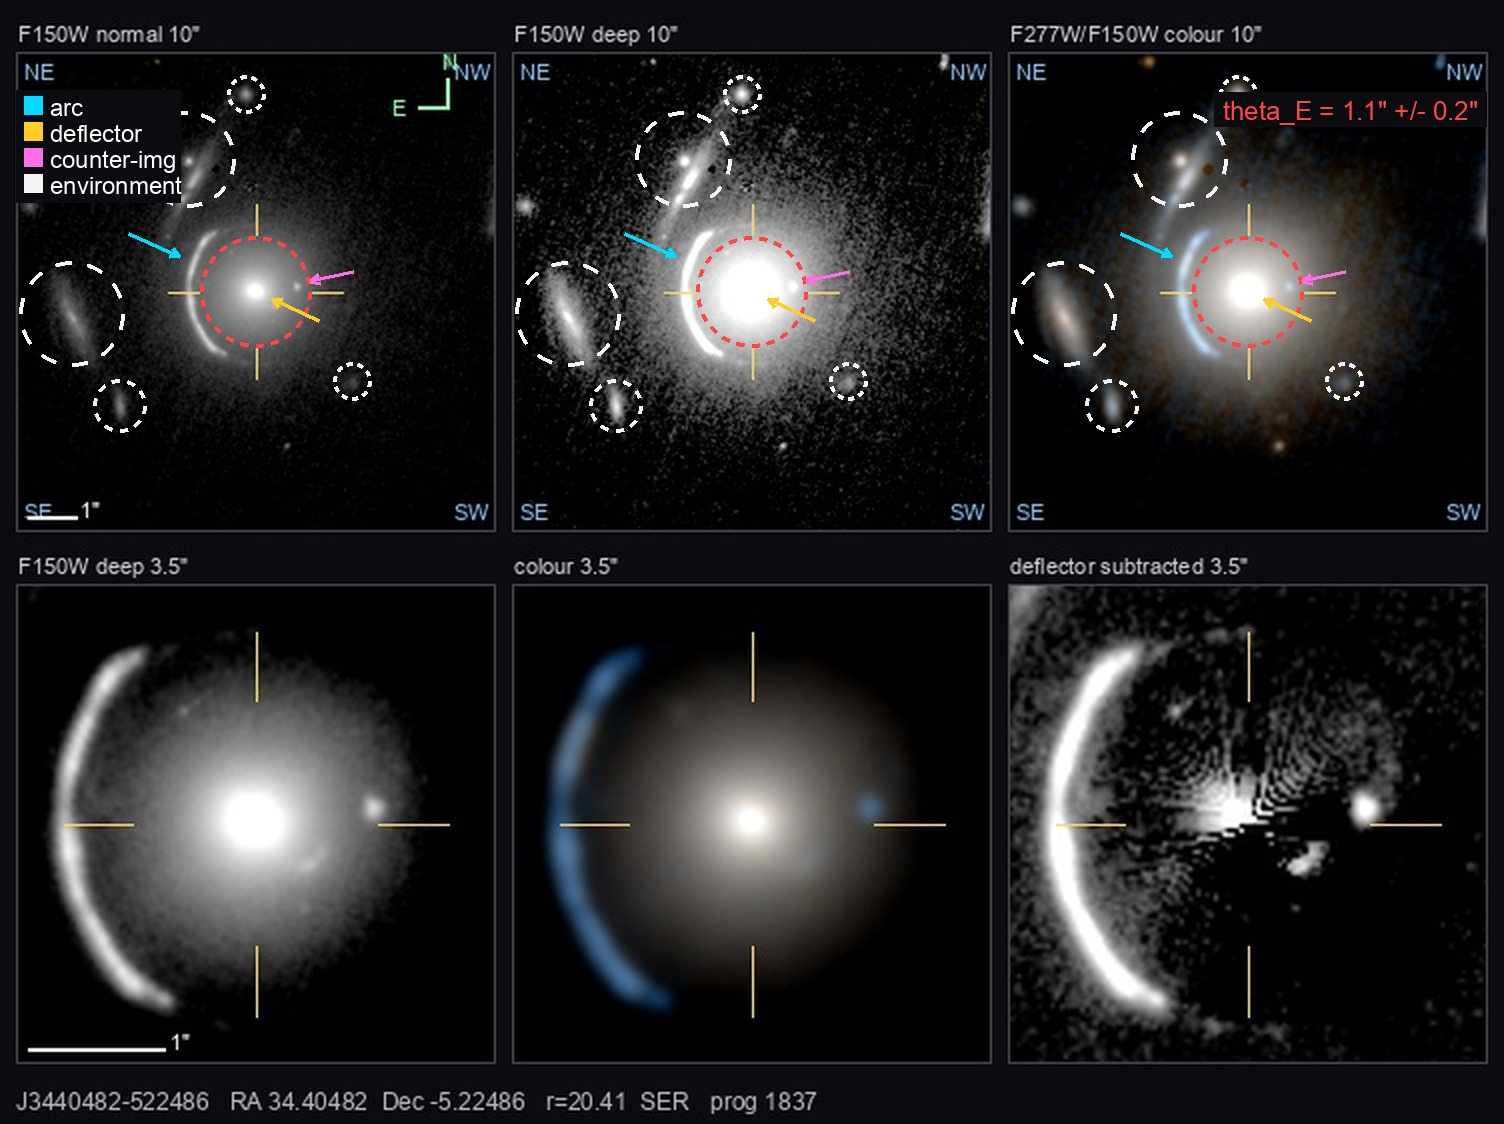
\includegraphics[width=0.9\linewidth]{figures/cand_J3440482-522486.jpg}
\caption{Rank 1, J3440482-522486 = SL2S\,J02176-0513, recovered blind at the
top of the ranking --- the validation anchor. Panels are the agent's own
annotated product: cyan = arc, yellow = deflector, magenta = counter-image,
white = environment galaxies, red dashed = blind \thetaE{}. Top row: $10''$
field (normal, deep, color); bottom row: $3.5''$ zoom (deep, color,
deflector-subtracted).}
\label{fig:rank1}
\end{figure}

\begin{figure}[ht]
\centering
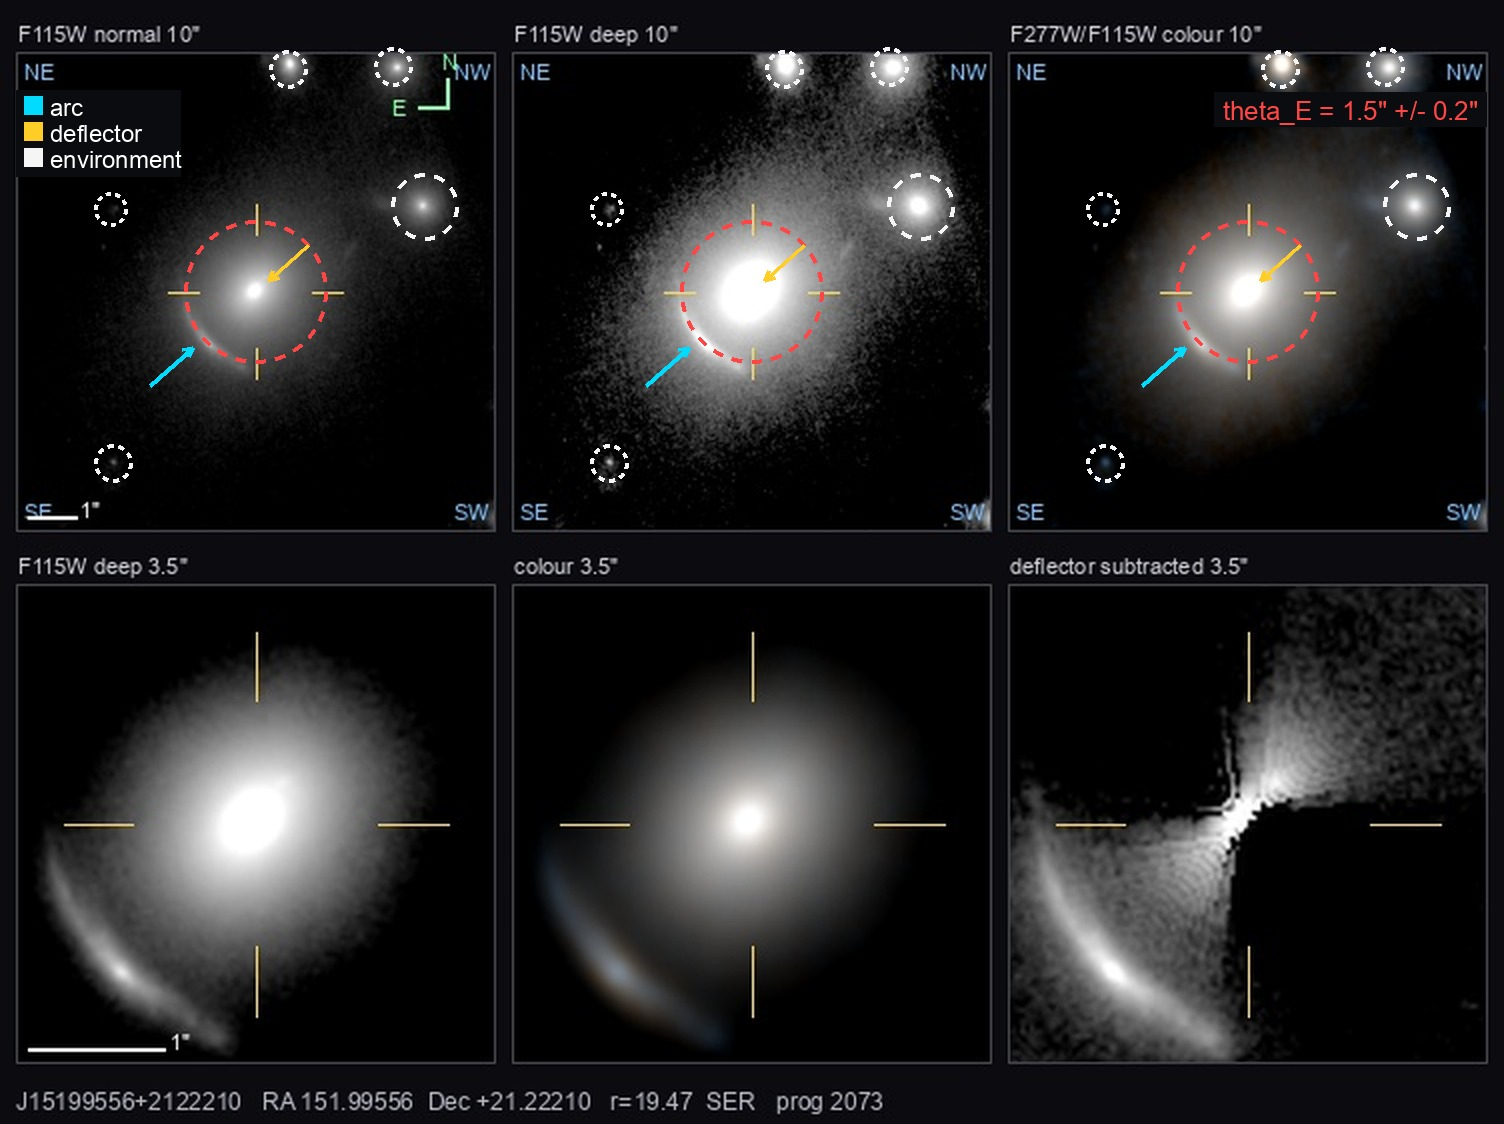
\includegraphics[width=0.9\linewidth]{figures/cand_J15199556+2122210.jpg}
\caption{Rank 2, J15199556+2122210: grade A, no prior identification found.
A thin blue arc at $r=1.45''\pm0.03''$ spanning $\sim$77$^\circ$ around a
$z_{\rm sp}=0.509$ elliptical (SDSS), in the JWST program 2073 field of the
$z=7.5$ quasar Poniu\={a}\v{e}na. Blind $\thetaE=1.48''\pm0.25''$.}
\label{fig:rank2}
\end{figure}

The two cleanest new galaxy-scale candidates are rank 2
(Figure~\ref{fig:rank2}) and rank 10 (J23069956+2559453; grade A,
$z_{\rm ph}=0.66$, blind $\thetaE=1.37''\pm0.25''$), both surviving all three
adversarial personas and carrying no prior identification in the audit.
Rank 8 (J16644236-1024898; grade B, $z_{\rm ph}=0.41$) is a strong
galaxy-scale configuration in the MACS J1105.7$-$1014 cluster core. We
additionally note rank 3 (J34707505-219476; grade A) as a spectacular arc that
the audit places $1.06'$ from the core of Abell 2537 with cataloged multiple
images $29''$ away --- almost certainly real lensing, but cluster-associated
and requiring a cluster-aware model rather than a galaxy-galaxy
interpretation. Spectroscopic confirmation of the arcs (none of the sources
has a redshift) is the required next step for all of these.

\subsection{A group-scale system: the BCG of WH\,J135810.5-105636}
\label{sec:gem}

\begin{figure}[ht]
\centering
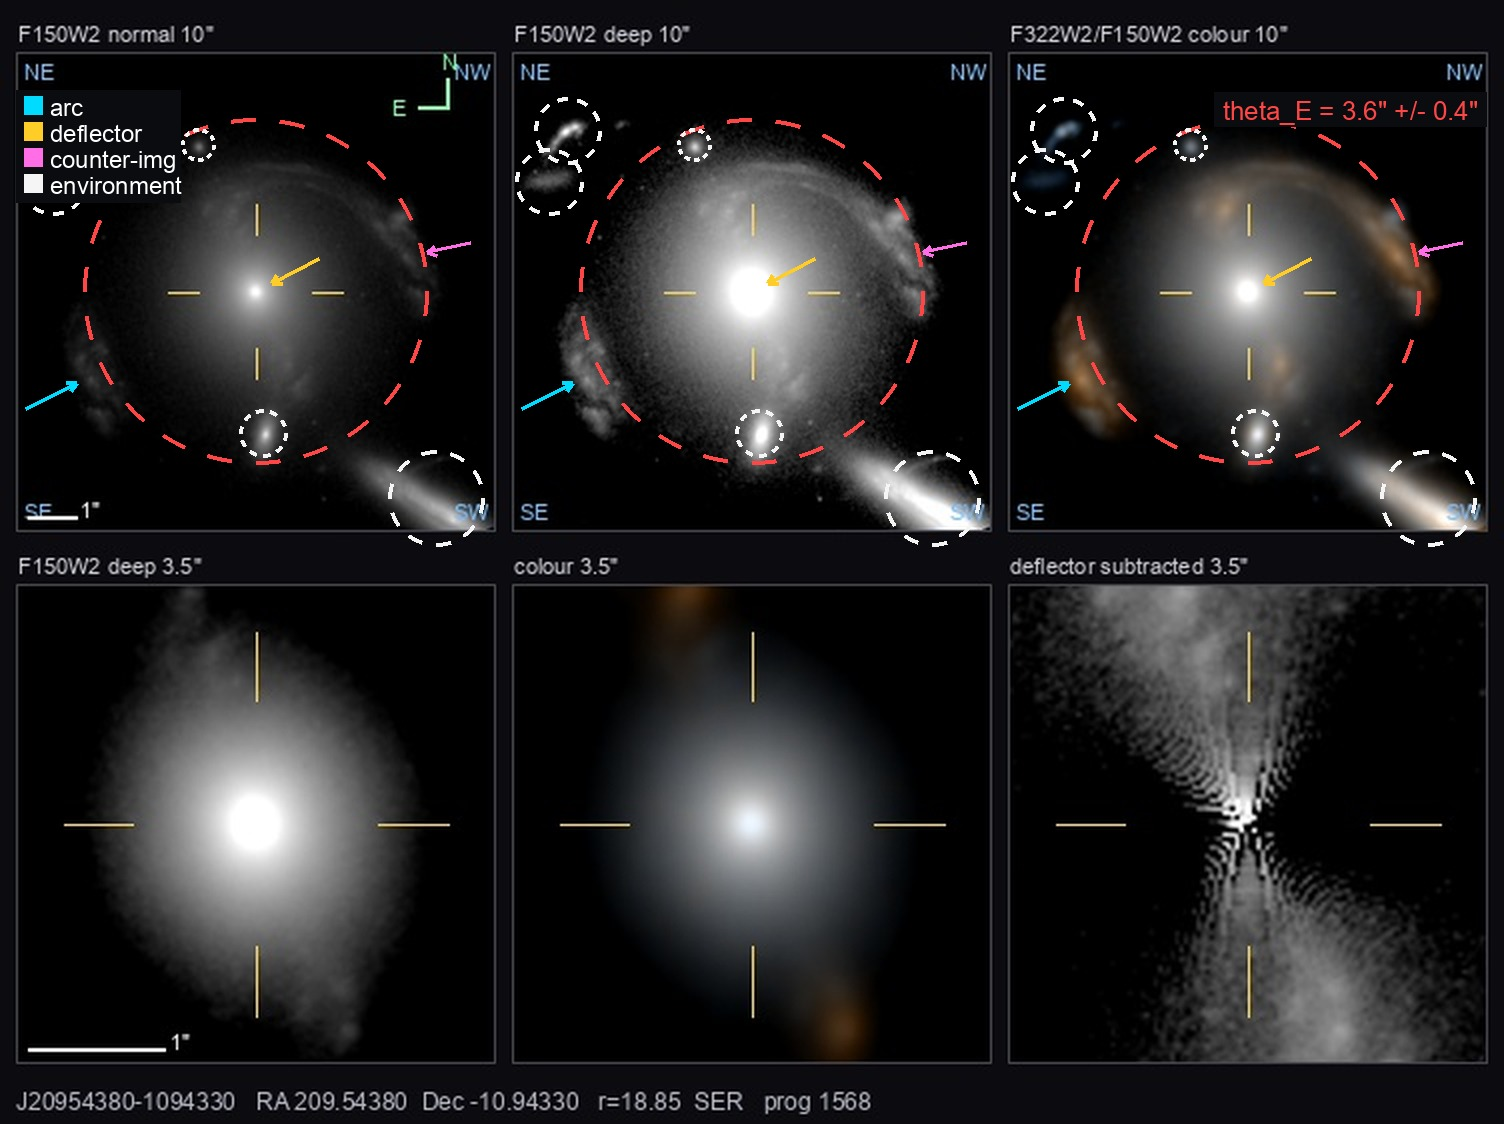
\includegraphics[width=0.9\linewidth]{figures/cand_J20954380-1094330.jpg}
\caption{Rank 15, J20954380-1094330 (grade C): a $\thetaE=3.6''\pm0.4''$
arc-plus-counter-arc system around the BCG of the \citet{wen2024catalog}
cluster WH\,J135810.5-105636 ($z_{\rm cl}=0.481$), in the 24.5\,ks
F150W2/F322W2 imaging of JWST calibration program 1568. The mirror-symmetric
arc pair (cyan/magenta) drives the blind \thetaE{}; the agent itself noted the
northern thin arc is \emph{not} concentric and excluded it from the estimate.}
\label{fig:gem}
\end{figure}

Rank 15 (Figure~\ref{fig:gem}) is the system flagged during our own review as
the most interesting single object in the list. The deflector
(RA, Dec $=209.5438^\circ, -10.9433^\circ$; $r=18.85$;
$z_{\rm ph}=0.495\pm0.026$, Legacy Surveys) coincides to $<$$0.1''$ with the
brightest cluster galaxy of WH\,J135810.5-105636, cluster ID 712636 in the
\citet{wen2024catalog} DESI Legacy Surveys cluster catalog at
$z_{\rm cl}=0.481$ --- a cluster catalogued from the same DECam imaging in
which the arcs are too faint to have been noticed, and absent from every lens
catalog the audit could reach. The measurement agents blindly traced a broad
eastern arc (ridge radius $3.87''$) and a mirror-symmetric northwestern
counter-arc ($3.36''$), both concave inward, giving
$\thetaE=3.6''\pm0.4''$ from half their separation.

Taking $z_l=0.481$ and the blind \thetaE{}, the Einstein radius is
$R_{\rm E}\simeq22$\,kpc and the enclosed projected mass is
\begin{equation}
M(<\thetaE) \;=\; \frac{c^2}{4G}\,\thetaE^2\,\frac{D_l D_s}{D_{ls}}
\;\approx\; (2.8\text{--}4.5)\times10^{12}\,\Msun
\quad (z_s = 1\text{--}3),
\label{eq:mass}
\end{equation}
corresponding to an SIS velocity dispersion of $\sim$420--530\,km\,s$^{-1}$
--- group-to-cluster scale, consistent with the low-richness Wen \& Han
identification. The arc morphology (broad, clumpy, with both blue knots and
orange material) led the geometry verifier to withhold full endorsement
(grade C), and its skepticism is recorded verbatim in the transcript:
morphologically the debris interpretation was not excludable from the panels
alone. A pixel-level lens model and source-redshift spectroscopy are the
decisive follow-ups; both are planned with collaborators.

\subsection{Data-quality caveats}\label{sec:caveats}

The audit surfaced defects that we report as part of the result. Ranks 7 and
14 are the same object $1.17''$ apart with different grades (B vs.\ C) ---
a deduplication miss across observations; ranks 16 and 17 are likely one
system counted twice ($8.78''$). One candidate has a null deflector photo-z.
The \code{candidate\_id} strings mangle coordinate precision and must not be
parsed as positions (the \code{ra\_sex}/\code{dec\_sex} columns are verified
to $0.008''$). Blind \thetaE{} values are geometric estimates from rendered
$8$-bit panels, not lens models; all color statements in verdicts are
composite-panel RGB ratios, not calibrated photometry. And every ``no prior
identification'' verdict carries the un-queried-SLED caveat. None of these
change the headline counts; all of them are exactly the kind of defect a
human referee should expect an agentic pipeline to produce silently, which is
why the independent audit exists.

% =============================================================================
\section{How the agent reasoned about lenses}\label{sec:reasoning}
% =============================================================================

The complete reasoning record of the campaign is preserved: 1{,}281 per-agent
JSONL transcripts (2.2\,GB) across 39 workflows, plus the three session-level
orchestration transcripts. Every record carries the model ID, timestamps, and
token usage; every tool call --- including every \code{Read} of a cutout image
--- is logged with its inputs. Two structural facts shape the analysis. First,
the model's private chain-of-thought is redacted in the transcripts, and its
conversational prose is thin (``I'll start by reading the batch file'');
essentially all scientific reasoning is externalized in the \emph{tool-call
payloads} --- the verdict JSON's \code{evidence}, \code{notes}, and
\code{alternative} fields and the end-of-batch structured summaries. Second,
because verdicts are structured, the corpus is quantitatively minable: the
statistics below are computed over all \numflagged{} evidence-bearing verdicts
and all 1{,}050 verification judgements.

\subsection{The inspection idiom}\label{sec:idiom}

Inspection evidence follows a stable five-part pattern, learned from nothing
more than the field-guide prompt:
(1) \emph{feature + offset + bearing} (``blue compact knot $\sim$$2.3''$ NW of
the red central galaxy''); (2) \emph{curvature and orientation relative to the
deflector} (``concave toward centre, at near-constant radius'');
(3) \emph{color relative to the host}; (4) \emph{persistence in the
deflector-subtracted panel}; and (5) an explicit \emph{self-caveat naming the
null hypothesis} (``caveat: nucleus shows strong 6-ray JWST diffraction
spikes, so a one-armed spiral / ring galaxy is not excluded''). Offsets are
consistently quoted to $0.1''$ read off the panel scale bar. Across the
flagged verdicts, the most frequent evidence terms are \emph{residual} (1{,}103
of \numflagged{} verdicts), \emph{knot} (1{,}039), \emph{blue} (777),
\emph{arc} (549), \emph{curved} (426), \emph{ring} (384), \emph{companion}
(344), \emph{concave} (305), and \emph{counter-image} (244) --- a vocabulary
indistinguishable from a human lens-search team's, deployed with positional
quantification on every claim.

\subsection{Calibration behavior: the shortlist, not the discovery}
\label{sec:calibration}

The screening prompt orders a high-recall pass, and the agents' verdict
distribution shows they internalized it to a degree we did not anticipate:
in the largest inspection workflow (60 batches, 840 verdicts), the agents
returned 523 \code{no}, 317 \code{likely}, and \emph{zero} \code{yes}, with a
self-imposed confidence ceiling of 50. Across the whole run, \code{yes}
appeared 14 times in \numinspected{} cutouts (0.26\%) --- and the highest
confidence of the entire campaign, 95, went to the cutout that is in fact
SL2S\,J02176-0513. The screening stage, in other words, behaves as a
shortlist generator that reserves assertion for overwhelming evidence, and
the burden of proof is carried by the adversarial stage
(Figure~\ref{fig:confidence}). The inverse is also true and is the pipeline's
key weakness: recovered known lenses came back at confidences 15--30,
indistinguishable from the bulk of the shortlist (Section~\ref{sec:completeness}).

\subsection{Verification argues by mechanism, and escalates to measurement}
\label{sec:verifiers}

Verifier language is different in kind from inspector language: rather than
describing features, it names generating mechanisms --- ``the classic bipolar
model-mismatch butterfly,'' ``S\'ersic-mismatch dipole,'' ``concentric-ripple
over-subtraction artefact,'' ``spindle-shaped edge-on galaxy'' --- and kills
candidates by radial-vs-tangential elongation, radius monotonicity, same-side
geometry, or color identity with the host. The forced \code{alternative} field
yields a machine-readable false-positive taxonomy over the 1{,}008 failed
judgements: spiral arms and host rings (386), tidal/merger debris (193),
chance alignments and companions (193), reduction and model artifacts (106),
edge-on disks (60), and diffraction/PSF effects (16) --- quantitatively
matching the confuser classes an experienced human inspector lists first.

The geometry persona did something the prompts did not request: it wrote
measurement code. Fifteen of fifteen final-pass geometry agents ran shell
commands, and eleven performed genuine quantitative image analysis --- one
agent built a reusable script that converts panel pixels to arcseconds, masks
the yellow astrometric ticks by RGB threshold, transforms to polar
coordinates about the deflector, thresholds at the 92nd percentile, and fits
a weighted algebraic circle to measure the arc radius, its radial scatter,
and the offset of the center of curvature from the deflector centroid.
A representative kill reads:

\begin{quote}\small\itshape
``Polar profiling about the nucleus shows the feature sweeps $\sim$200\,deg
with its ridge radius growing monotonically from $1.43''$ at NW to $2.65''$
at SW, is $\sim$$0.7''$ wide radially, \ldots{} and has no counterpart
anywhere from E through S --- a winding arm, not a constant-radius tangential
arc.'' \normalfont(geometry persona, fail; alternative: ``inner ring /
winding spiral arm in the host lenticular's own disk'')
\end{quote}

\noindent and a representative pass, for what became rank 10:

\begin{quote}\small\itshape
``A thin tangential arc runs SE-through-S at $r\sim1.3''$ concave toward the
core with its centre of curvature on the deflector centroid, it is measurably
bluer than the halo at the same radius on the opposite side (R/B 1.13 vs
1.46) \ldots{} though no compact counter-image is resolved.''
\end{quote}

Inspection agents, by contrast, stayed almost purely visual, escalating only
as far as self-directed crop-and-zoom (31 of 99 agents in the sampled
workflow re-rendered ambiguous panels at higher magnification before
deciding). The escalation gradient --- visual screening, mechanistic
refutation, quantitative measurement --- emerged from the personas' goals,
not from explicit instruction, and it concentrated the expensive analysis
exactly where it mattered: candidates that survived it are the grade-A list.
Persona disagreement is preserved too: rank 21, the published lens
MACS0416-GGL1, passed morphology (``a smooth red DEV host \ldots{} has no
disk or spiral structure capable of hosting star-forming knots, so my
morphology attack cannot dispose of it'') while the artifact persona returned
\code{uncertain} --- the two verdicts, side by side, read like a referee
exchange. Extended excerpts, with transcript file paths for every quote, are
in Appendix~\ref{app:excerpts}.

\subsection{Literature agents and their discoveries about the tools}
\label{sec:litagents}

The per-candidate literature agents were the most tool-diverse: coordinate
conversion in shell, web search on both coordinate forms, NED and SIMBAD cone
searches, VizieR TAP, program identification, and --- when a survey paper
seemed relevant --- fetching the PDF and grepping its text. Their verdicts
draw exactly the distinction the audit later formalized: ``that cluster IS a
published cluster lens --- but its published arc is $23.2''$ away and its BCG
is $13.9''$ away, so this specific galaxy is not the published deflector.''
The audit session's own findings double as a field report on the state of the
infrastructure: \code{astroquery}'s NED module wraps a CGI endpoint that
times out where NED's TAP service answers in a second; SIMBAD's primary
\code{otype} misses lenses typed as radio galaxies unless the \code{otypes}
table is queried; and naive VizieR matching against everything with ``lens''
in the title would have matched the RELICS \emph{source} catalog and marked
every candidate in those fields as known. Each of these is a silent
false-negative or false-positive channel for any automated crossmatch, found
because the agents' failures were inspectable.

\subsection{What the corpus does not show}\label{sec:limits-reasoning}

The transcripts also delimit the modality's current ceiling. No agent
performed calibrated photometry or touched FITS pixels --- all judgements,
including the quantitative ones, operate on rendered 8-bit panels. No agent
proposed a lens model. The redacted chain-of-thought means we characterize
the reasoning by its externalized artifacts, not its internal process. And
the duplicate-candidate defects of Section~\ref{sec:caveats} passed through
every stage unremarked: each agent sees only its assignment, and nothing in
the architecture owns global consistency. These are not fundamental limits
--- FITS-native tooling, modeling subagents, and a consistency pass are all
straightforward extensions --- but they mark where human oversight was, and
remains, load-bearing.

% =============================================================================
\section{Discussion}\label{sec:discussion}
% =============================================================================

\subsection{Against the existing discovery modalities}\label{sec:compare}

The relevant comparison classes are CNN searches on uniform surveys and
expert/citizen visual campaigns. Against CNNs
\citep{huang2020finding,huang2021discovering,storfer2024new,inchausti2025strong,
petrillo2017finding,jacobs2019extended}, the agentic search needed \emph{no
training set} --- which is what made the heterogeneous JWST archive
addressable at all --- and it emits, for every candidate, an evidence
paragraph, a named-alternative record, and a literature verdict that a human
can adjudicate line by line. Its per-object cost ($\sim$5{,}200 tokens to
inspect, $\sim$21{,}000 per verification judgement) is orders of magnitude
above a CNN forward pass, and its throughput (5{,}308 cutouts in a working
day, subscription-throttled) is orders of magnitude below a survey sweep; at
DESI-survey scale ($10^7$--$10^8$ galaxies) this modality, today, is not a
replacement but a \emph{complement}: the natural division of labor is CNNs
for uniform breadth and agents for heterogeneous archives, hard tails, and
candidate adjudication. Against visual campaigns
\citep{marshall2016spacewarps,garvin2022hubble,mahler2025cowls2}, the agent's
48--54\% single-pass recall at COWLS-like depth is below expert performance
on comparable imaging, but it is measured, repeatable, improvable by
prompt-level alignment --- and it took two days, not a campaign season.

Two further properties have no analog in either modality. First,
\emph{auditability}: the 2.2\,GB transcript corpus is a complete causal
record; every claim in the top-100 table can be traced to the images an agent
read and the words it wrote. CNN saliency maps and volunteer click streams do
not support this kind of retrospective cross-examination. Second,
\emph{closed-loop literature awareness}: the same system that found the
candidates also determined, with documented queries, which were already
known --- a step that in conventional pipelines is a separate, human-driven
project.

\subsection{The honest failure modes}\label{sec:failures}

Our own expert review of the top 100, conducted on the contact sheet before
the audit, identified four false-positive families: mergers, spiral/ring
galaxies, image-reduction artifacts, and busy cluster fields. The
verification stage's own alternative-explanation taxonomy
(Section~\ref{sec:verifiers}) names the same families, and the audit adds the
fifth failure that neither stage owned: novelty overstatement in cluster
fields. The completeness numbers are the sharpest limitation --- a 92\%
verification false-rejection rate on known lenses means the grade system is a
purity instrument only --- and the weak confidence calibration means the
ranking below the verified tier is ``worth a look,'' not a probability. All
of these are measured, not anecdotal, which is what makes the next iteration
tractable.

\subsection{The human-alignment loop}\label{sec:alignment}

The natural next experiment is already designed: split the graded top-100
(and the recovered-known set) into alignment and validation halves with
matched lens counts; feed the alignment half's expert annotations --- which
FPs fooled which persona, which real arcs the geometry checker under-weighted,
which residual-panel artifacts recur --- back into the inspection and
verification prompts; and re-run on the validation half to measure the purity
and completeness deltas. Because the ``model'' here is a prompt stack rather
than trained weights, the alignment cycle costs hours, is fully documented in
version control, and is legible to the domain experts driving it. A second
extension, Phase B of the original plan, is JWST-native target selection
(dropping the Legacy Surveys $r<21$ elliptical prior) to reach high-redshift
and spiral deflectors --- the regime where the archive's depth is unique and
where COWLS \citep{nightingale2025cowls1} shows the yield lives.

\subsection{Reproducibility}\label{sec:repro}

The run is re-executable from its repository (pipeline scripts, workflow
definitions, prompts, manifests) against the same public archive, and its
conclusions are re-derivable from the preserved verdict files without any
model access. Exact re-generation of verdicts is not expected --- the model
samples, usage limits reshuffle batches, and the hosted model version will
drift --- so we treat reproducibility at the level that matters
scientifically: the candidate list, the control-recovery numbers, and every
quoted excerpt are checked against the archived artifacts, and the audit
re-derived the novelty claims independently. Pinning open-weight models or
logging seeds would tighten this further; transcript preservation is, for
now, the strongest reproducibility instrument this modality has.

% =============================================================================
\section{Conclusions}\label{sec:conclusions}
% =============================================================================

A single natural-language request --- find strong lenses in the public JWST
archive and show me the top 100 --- was carried by a general-purpose agentic
AI through pipeline design, live interface verification, code, census,
streaming cutouts, exhaustive vision inspection with blind controls,
three-persona adversarial verification, blind Einstein-radius measurement,
literature crossmatching, and report generation, in about two days of
wall-clock on a consumer subscription. The output is not a black-box score:
it is a ranked, evidenced, literature-annotated candidate list with a
complete audit trail.

Measured against that record: the pipeline re-found real lenses blind (SL2S
J02176-0513 at rank 1 with the campaign's highest confidence; 10 published
systems in the top 100), delivered at least two clean new grade-A
galaxy-scale candidates (ranks 2 and 10) and a group-scale arc system around
a WH cluster BCG with $\thetaE=3.6''$ (rank 15), recovered 48\% of
blind-injected COWLS controls and 54\% of 239 catalogued lenses in its
footprint, and overclaimed novelty in cluster fields until an independent
audit corrected it. The transcript corpus shows a division of cognitive labor
that no one prompted in detail: a screening pass that hedges, an adversarial
pass that argues by named mechanism and invents its own measurement code, and
literature agents that distinguish a lensing cluster from a lensed galaxy.

Strong-lens discovery has scaled, in turn, by eyes, by crowds, and by
convolutional filters. This experiment demonstrates a fourth modality ---
by argument: agents that look, measure, refute, and cite, leaving a record a
referee can check. Its present completeness is modest and measured; its
alignment loop is fast and human-legible; and the archive it opens ---
everything public, heterogeneous, and too irregular to train on --- is
precisely the data no other modality serves.

% =============================================================================
\section*{Software and data availability}
% =============================================================================
\addcontentsline{toc}{section}{Software and data availability}

The complete pipeline (scripts \code{01}--\code{20}, workflow definitions
with all prompts, and the session-level transcripts) and all result tables
(\code{results.csv} for all \numtargets{} targets, the top-100 master table,
control-recovery and known-lens-recovery tables, and the annotated candidate
documents) are at
\url{https://github.com/kvinneslandn-ML-AI/jwst-strong-lens-search}. The
1{,}281 per-agent transcripts (2.2\,GB uncompressed) are archived alongside
this paper's analysis scripts in the project repository
(\code{reproductions/agentic-lens-discovery/}); a Zenodo deposit is planned
at submission. JWST data are from the public MAST archive
(\code{stpubdata}); deflector catalogs and photometric redshifts from the
DESI Legacy Imaging Surveys DR9/DR10 \citep{dey2019overview,zhou2021clustering};
positive controls from COWLS \citep{nightingale2025cowls1}.

\software{\cc{} v2.1.224 \citep{anthropic2025claudecode} running
\texttt{claude-opus-5} \citep{anthropic2026opus}; \code{astropy}
\citep{astropy2022}, \code{astroquery}, \code{fsspec}, \code{numpy},
\code{scipy}, \code{matplotlib}, \code{pandas}, \code{Pillow}.}

\facilities{JWST (NIRCam), MAST, Blanco/DECam (Legacy Surveys), Astro Data
Lab, CDS (SIMBAD, VizieR), NED.}

% =============================================================================
\begin{acknowledgments}
% =============================================================================
We thank Saul Perlmutter for the suggestion of the split-half alignment
validation design, and Aniket [surname] and Sean [surname] for discussions on
lens modeling of the rank-15 system. % TODO confirm names/consent
The search itself was executed by \cc{} agents; all scientific claims were
verified by the authors, and the independent novelty audit was run separately
from the discovery session. This work used public data from JWST (operated by
AURA under NASA contract NAS5-03127) and the DESI Legacy Imaging Surveys.
\end{acknowledgments}

% =============================================================================
\appendix
% =============================================================================

\section{The top-100 candidate list}\label{app:top100}

Figure~\ref{fig:contact} shows the full contact sheet; Table~\ref{tab:top100}
lists all 100 candidates. Machine-readable versions, including the evidence
and note text for every candidate, are in the data repository.

\begin{figure}[p]
\centering
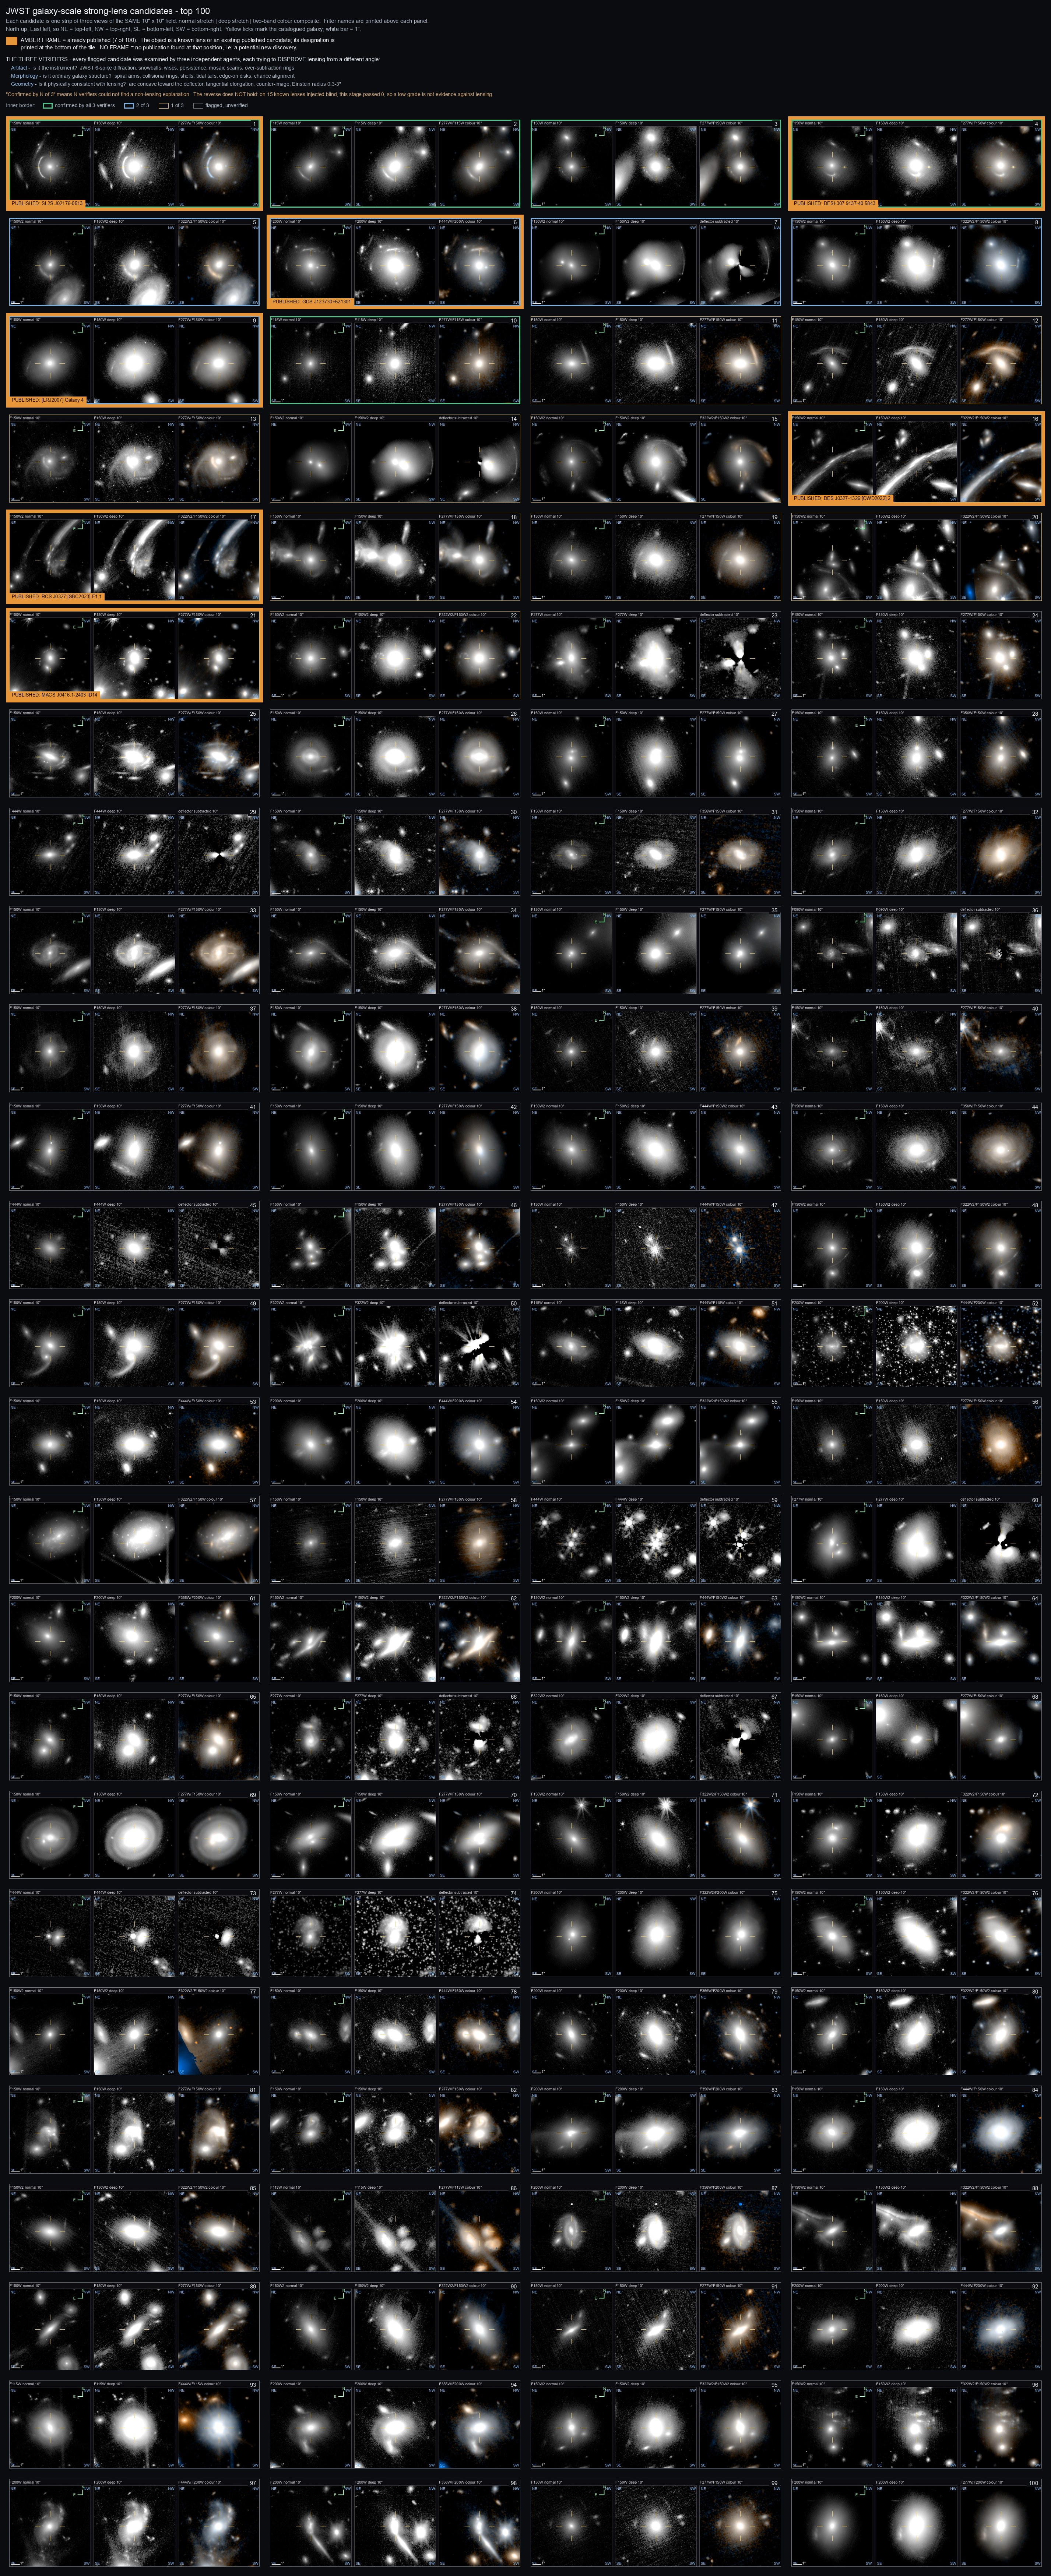
\includegraphics[height=0.86\textheight,keepaspectratio]{figures/contact_sheet.jpg}
\caption{All 100 ranked candidates, one three-panel strip each (normal
stretch, deep stretch, color composite). Border color encodes the verifier
tier (green: 3/3; blue: 2/3; thin blue: 1/3; gray: flagged, unverified);
amber matting marks systems the crossmatch found already published. A
full-resolution version is in the data repository.}
\label{fig:contact}
\end{figure}

% Auto-generated by assets/analysis/make_appendix_table.py — do not edit.
\begin{scriptsize}
\setlength{\tabcolsep}{2pt}
\begin{longtable}{@{}rlllcccclc@{}}
\caption{The top-100 candidate list. $\theta_{\mathrm{E}}$ is the blind geometric estimate (arc radius or half image-separation) measured from the imaging alone; grades: A = passed all three adversarial verifiers, B = two, C = one, U = flagged but not selected for verification. ``Prior ID'' is the run's own literature verdict; the independent audit (Section~\ref{sec:results-xmatch}) further reclassifies 24 rows as cluster-field matches. Exposure time is the SW-filter total.}\label{tab:top100}\\
\toprule
\# & ID & RA, Dec (J2000) & Grade & $\theta_{\mathrm{E}}$ ($''$) & $z_{\rm ph}$ & $z_{\rm sp}$ & Filters & $t_{\rm exp}$ (ks) & Prior ID\\
\midrule
\endfirsthead
\toprule
\# & ID & RA, Dec (J2000) & Grade & $\theta_{\mathrm{E}}$ ($''$) & $z_{\rm ph}$ & $z_{\rm sp}$ & Filters & $t_{\rm exp}$ (ks) & Prior ID\\
\midrule
\endhead
\midrule \multicolumn{10}{r}{\emph{continued}}\\ \bottomrule
\endfoot
\bottomrule
\endlastfoot
1 & J3440482-522486 & 02:17:37.156, -05:13:29.49 & A & 1.15$\pm$0.20 & 0.697 & 0.6460 & F150W/F277W & 22.6 & published\\
2 & J15199556+2122210 & 10:07:58.936, +21:13:19.57 & A & 1.48$\pm$0.25 & 0.517 & 0.5094 & F115W/F277W & 7.5 & none found\\
3 & J34707505-219476 & 23:08:18.011, -02:11:41.13 & A & 1.40$\pm$0.30 & 0.305 & -- & F150W/F277W & 1.2 & none found\\
4 & J30791374-4058431 & 20:31:39.299, -40:35:03.50 & A & 1.12$\pm$0.25 & 0.562 & -- & F150W/F277W & 1.2 & published\\
5 & J34084513-960342 & 22:43:22.831, -09:36:12.31 & B & 1.35$\pm$0.20 & 0.443 & -- & F150W2/F322W2 & 1.8 & none found\\
6 & J18937456+6221686 & 12:37:29.894, +62:13:00.71 & B & 2.10$\pm$0.35 & 0.497 & -- & F200W/F444W & 5.8 & published\\
7 & J18030075+2309921 & 12:01:12.180, +23:05:57.16 & B & 4.00$\pm$0.40 & 0.293 & -- & F150W2 & 1.8 & none found\\
8 & J16644236-1024898 & 11:05:46.167, -10:14:56.32 & B & 2.15$\pm$0.25 & 0.407 & -- & F150W2/F322W2 & 1.8 & none found\\
9 & J19789495-132348 & 13:11:34.789, -01:19:24.52 & B & 2.70$\pm$0.40 & 0.189 & -- & F150W/F277W & 7.5 & published\\
10 & J23069956+2559453 & 15:22:47.895, +25:35:40.30 & A & 1.37$\pm$0.25 & 0.656 & -- & F115W/F277W & 1.9 & none found\\
11 & J8999381-2012203 & 05:59:58.513, -20:07:19.32 & C & 2.00$\pm$0.30 & 0.261 & -- & F150W/F277W & 3.3 & none found\\
12 & J2451534-2191925 & 01:38:03.683, -21:55:09.29 & C & 2.24$\pm$0.35 & 0.373 & -- & F150W/F277W & 1.0 & none found\\
13 & J18805344+1121596 & 12:32:12.825, +11:12:57.45 & C & 0.72$\pm$0.20 & 0.518 & 0.5440 & F150W/F277W & 1.5 & none found\\
14 & J18030108+2309932 & 12:01:12.259, +23:05:57.56 & C & 4.60$\pm$0.35 & 0.266 & -- & F150W2 & 1.8 & none found\\
15 & J20954380-1094330 & 13:58:10.511, -10:56:35.88 & C & 3.60$\pm$0.40 & 0.495 & -- & F150W2/F322W2 & 24.5 & none found\\
16 & J5186648-1343587 & 03:27:27.956, -13:26:09.12 & C & 17.60$\pm$3.00 & 1.431 & -- & F150W2/F322W2 & 1.8 & published\\
17 & J5186803-1343778 & 03:27:28.328, -13:26:16.01 & C & -- & 0.918 & -- & F150W2/F322W2 & 1.8 & published\\
18 & J4006002-161474 & 02:40:14.406, -01:36:53.07 & C & 0.81$\pm$0.20 & 0.595 & -- & F150W/F277W & 10.3 & none found\\
19 & J33372744-1401097 & 22:14:54.585, -14:00:39.48 & C & 2.50$\pm$0.50 & 0.478 & -- & F150W/F277W & 1.2 & none found\\
20 & J710586-7562357 & 00:28:25.406, -75:37:24.84 & C & -- & 0.587 & -- & F150W2/F322W2 & 1.8 & none found\\
21 & J6403415-2406677 & 04:16:08.196, -24:04:00.39 & C & 1.20$\pm$0.30 & 0.455 & -- & F150W/F277W & 37.1 & published\\
22 & J5414235-4704895 & 03:36:34.163, -47:02:56.20 & C & 1.70$\pm$0.40 & 0.655 & -- & F150W2/F322W2 & 1.8 & none found\\
23 & J18818168+1282960 & 12:32:43.604, +12:49:46.56 & U & -- & 0.482 & 0.4659 & F277W & -- & none found\\
24 & J6439169-1191885 & 04:17:34.005, -11:55:07.87 & U & 2.80$\pm$0.50 & 0.428 & -- & F150W/F277W & 6.4 & none found\\
25 & J3996679-159719 & 02:39:52.029, -01:35:49.89 & U & 1.60$\pm$0.35 & 0.346 & -- & F150W/F277W & 37.1 & field\\
26 & J357850-3044809 & 00:14:18.841, -30:26:53.11 & U & 2.45$\pm$0.40 & 0.323 & -- & F150W/F277W & 21.3 & none found\\
27 & J15032484+248405 & 10:01:17.961, +02:29:02.59 & U & 0.83$\pm$0.25 & 0.345 & 0.3486 & F150W/F277W & 1.0 & none found\\
28 & J26831233+6515810 & 17:53:14.959, +65:09:29.17 & U & 1.18$\pm$0.25 & 0.577 & -- & F150W/F356W & 33.6 & none found\\
29 & J20148636+4809579 & 13:25:56.726, +48:05:44.85 & U & 2.70$\pm$0.60 & 0.439 & -- & F444W & -- & none found\\
30 & J9006236-2015944 & 06:00:14.967, -20:09:34.00 & U & 2.50$\pm$0.40 & 0.934 & -- & F150W/F277W & 5.0 & none found\\
31 & J26876212+6510625 & 17:55:02.910, +65:06:22.51 & U & 0.60$\pm$0.20 & 0.348 & -- & F150W/F356W & 7.8 & none found\\
32 & J804181+1819597 & 00:32:10.034, +18:11:45.49 & U & -- & 0.394 & -- & F150W/F277W & 2.5 & none found\\
33 & J32232919-763201 & 21:29:19.006, -07:37:55.24 & U & -- & 0.731 & -- & F150W/F277W & 1.2 & none found\\
34 & J17771210-2809562 & 11:50:50.904, -28:05:44.23 & U & -- & 0.402 & -- & F150W/F277W & 2.5 & possible\\
35 & J3807110-4434755 & 02:32:17.064, -44:20:51.19 & U & 0.38$\pm$0.20 & 0.272 & -- & F150W/F277W & 1.2 & none found\\
36 & J15055009+250185 & 10:02:12.021, +02:30:06.65 & U & -- & 0.476 & 0.5799 & F090W & 1.2 & none found\\
37 & J15009907+202286 & 10:00:23.777, +02:01:22.31 & U & 3.30$\pm$0.45 & 0.422 & 0.4619 & F150W/F277W & 2.7 & none found\\
38 & J15010748+230270 & 10:00:25.796, +02:18:09.71 & U & 1.15$\pm$0.35 & 0.229 & 0.2199 & F150W/F277W & 22.0 & none found\\
39 & J16305610+3001292 & 10:52:13.464, +30:00:46.50 & U & 1.30$\pm$0.35 & 0.145 & -- & F150W/F277W & 2.1 & none found\\
40 & J15029814+254087 & 10:01:11.554, +02:32:27.15 & U & 1.60$\pm$0.40 & 0.193 & 0.1116 & F150W/F277W & 1.0 & none found\\
41 & J34708849-217825 & 23:08:21.237, -02:10:41.71 & U & 0.95$\pm$0.30 & 0.252 & -- & F150W/F277W & 1.2 & none found\\
42 & J12411163+1923209 & 08:16:26.791, +19:13:55.52 & U & 1.90$\pm$0.40 & 0.333 & -- & F150W/F277W & 5.3 & none found\\
43 & J15049363+206401 & 10:01:58.471, +02:03:50.44 & U & -- & 0.558 & 0.5469 & F150W2/F444W & 18.9 & none found\\
44 & J26807645+6520932 & 17:52:18.348, +65:12:33.55 & U & 0.98$\pm$0.30 & 0.591 & -- & F150W/F356W & 33.6 & none found\\
45 & J8570140-2144889 & 05:42:48.335, -21:26:56.00 & U & 1.70$\pm$0.40 & 0.116 & -- & F444W & -- & none found\\
46 & J9002960-2014057 & 06:00:07.104, -20:08:26.04 & U & 1.10$\pm$0.30 & 0.418 & -- & F150W/F277W & 5.0 & none found\\
47 & J15069997+222588 & 10:02:47.993, +02:13:33.15 & U & -- & 0.316 & -- & F150W/F444W & 2.2 & none found\\
48 & J4312165-2100739 & 02:52:29.196, -21:00:26.60 & U & 2.05$\pm$0.25 & 0.653 & -- & F150W2/F322W2 & 1.8 & field\\
49 & J5282421-774282 & 03:31:17.811, -07:44:34.15 & U & -- & 0.380 & -- & F150W/F277W & 1.0 & none found\\
50 & J20945435-1082161 & 13:57:49.043, -10:49:17.80 & U & 0.52$\pm$0.20 & -- & -- & F322W2 & -- & none found\\
51 & J4310830-518328 & 02:52:25.993, -05:10:59.81 & U & -- & 0.316 & -- & F115W/F444W & 2.2 & none found\\
52 & J14920654+6969086 & 09:56:49.570, +69:41:27.09 & U & -- & 0.306 & -- & F200W/F444W & 75.8 & none found\\
53 & J15067319+221999 & 10:02:41.566, +02:13:11.98 & U & -- & 0.310 & 0.3054 & F150W/F444W & 2.2 & none found\\
54 & J4784995-5841089 & 03:11:23.988, -58:24:39.21 & U & 1.60$\pm$0.40 & 0.390 & -- & F200W/F444W & 7.9 & none found\\
55 & J4205283+264369 & 02:48:12.679, +02:38:37.29 & U & 1.35$\pm$0.35 & 0.561 & -- & F150W2/F322W2 & 1.8 & none found\\
56 & J14977486+224978 & 09:59:05.966, +02:14:59.21 & U & 1.46$\pm$0.35 & 0.457 & 0.3895 & F150W/F277W & 1.0 & none found\\
57 & J21006317+1456150 & 14:00:15.160, +14:33:41.40 & U & 2.17$\pm$0.45 & 1.231 & -- & F150W/F322W2 & 113.4 & none found\\
58 & J2235243-7358297 & 01:29:24.583, -73:34:58.70 & U & -- & 0.450 & -- & F150W/F277W & 1.3 & none found\\
59 & J3419795-502846 & 02:16:47.507, -05:01:42.45 & U & 1.17$\pm$0.40 & 0.257 & -- & F444W & -- & none found\\
60 & J20960149-304690 & 13:58:24.358, -03:02:48.85 & U & 1.50$\pm$0.35 & 0.273 & -- & F277W & -- & none found\\
61 & J8149689-2410706 & 05:25:59.254, -24:06:25.43 & U & -- & 0.714 & -- & F200W/F356W & 2.8 & none found\\
62 & J15261689-1266966 & 10:10:28.052, -12:40:10.77 & U & 1.25$\pm$0.30 & 0.517 & -- & F150W2/F322W2 & 1.8 & none found\\
63 & J15067092+210603 & 10:02:41.021, +02:06:21.72 & U & 1.65$\pm$0.35 & 0.329 & 0.3392 & F150W2/F444W & 18.9 & none found\\
64 & J20865088+7724666 & 13:54:36.212, +77:14:47.96 & U & 1.25$\pm$0.40 & 0.410 & -- & F150W2/F322W2 & 1.8 & none found\\
65 & J4429240-2347200 & 02:57:10.177, -23:28:19.21 & U & 1.55$\pm$0.40 & 0.537 & -- & F150W/F277W & 1.2 & none found\\
66 & J18850875+1133833 & 12:34:02.101, +11:20:17.98 & U & 1.28$\pm$0.35 & 0.499 & -- & F277W & -- & none found\\
67 & J20948181-1096952 & 13:57:55.633, -10:58:10.27 & U & -- & 0.358 & -- & F322W2 & -- & none found\\
68 & J17772978-2808033 & 11:50:55.148, -28:04:49.20 & U & 2.46$\pm$0.40 & 0.387 & -- & F150W/F277W & 2.5 & none found\\
69 & J18931633+6219972 & 12:37:15.919, +62:11:59.00 & U & 0.89$\pm$0.35 & 0.108 & -- & F150W/F277W & 5.7 & none found\\
70 & J17174762+4246955 & 11:26:59.428, +42:28:10.39 & U & 0.66$\pm$0.25 & 0.351 & -- & F150W/F277W & 1.9 & none found\\
71 & J12391133+1822895 & 08:15:38.720, +18:13:44.23 & U & 1.66$\pm$0.45 & 0.533 & -- & F150W2/F322W2 & 8.6 & none found\\
72 & J21007480+1455269 & 14:00:17.951, +14:33:09.70 & U & 1.31$\pm$0.30 & 0.480 & -- & F150W/F322W2 & 113.4 & none found\\
73 & J8575205-2143155 & 05:43:00.492, -21:25:53.57 & U & 1.10$\pm$0.35 & 0.450 & -- & F444W & -- & none found\\
74 & J16193787+1252943 & 10:47:45.088, +12:31:45.96 & U & 1.55$\pm$0.40 & 0.459 & -- & F277W & -- & none found\\
75 & J35084320-3043955 & 23:23:22.368, -30:26:22.40 & U & 0.73$\pm$0.30 & 0.342 & -- & F200W/F322W2 & 5.0 & none found\\
76 & J8732838-6207334 & 05:49:18.810, -62:04:24.03 & U & 2.50$\pm$0.40 & 0.408 & -- & F150W2/F322W2 & 1.8 & none found\\
77 & J9192602-4479623 & 06:07:42.246, -44:47:46.44 & U & 1.45$\pm$0.35 & 0.232 & -- & F150W2/F322W2 & 1.8 & none found\\
78 & J18895415+499333 & 12:35:48.996, +04:59:35.98 & U & -- & 0.592 & -- & F150W/F444W & 74.7 & none found\\
79 & J16456132+2953030 & 10:58:14.717, +29:31:49.06 & U & 2.96$\pm$0.60 & 0.494 & -- & F200W/F356W & 2.8 & none found\\
80 & J15424410+3903685 & 10:16:58.583, +39:02:12.65 & U & 1.39$\pm$0.35 & 0.653 & -- & F150W2/F322W2 & 1.8 & none found\\
81 & J31352710-005281 & 20:54:06.504, -00:03:10.11 & U & -- & 0.258 & -- & F150W/F277W & 7.5 & none found\\
82 & J21483295+5282544 & 14:19:19.907, +52:49:31.57 & U & 2.30$\pm$0.40 & 0.387 & 0.3537 & F150W/F277W & 2.8 & none found\\
83 & J3470183+013617 & 02:18:48.440, +00:08:10.23 & U & -- & 0.205 & -- & F200W/F356W & 2.8 & none found\\
84 & J15057245+223798 & 10:02:17.387, +02:14:16.73 & U & -- & 0.102 & 0.1248 & F150W/F444W & 2.2 & none found\\
85 & J20861957+7726170 & 13:54:28.697, +77:15:42.12 & U & 2.00$\pm$0.35 & 0.419 & -- & F150W2/F322W2 & 1.8 & none found\\
86 & J21518078+5278672 & 14:20:43.388, +52:47:12.19 & U & -- & 0.444 & -- & F115W/F277W & 2.8 & none found\\
87 & J26816024+6505016 & 17:52:38.458, +65:03:00.59 & U & 0.82$\pm$0.30 & 0.640 & -- & F200W/F356W & 31.1 & none found\\
88 & J32840780+1769774 & 21:53:37.871, +17:41:51.85 & U & 1.45$\pm$0.35 & 0.272 & -- & F150W2/F322W2 & 1.8 & none found\\
89 & J9003772-2015513 & 06:00:09.053, -20:09:18.48 & U & 1.15$\pm$0.35 & 0.364 & -- & F150W/F277W & 3.3 & none found\\
90 & J1637643+1340558 & 01:05:30.343, +13:24:20.10 & U & 2.70$\pm$0.45 & 0.216 & -- & F150W2/F322W2 & 1.8 & none found\\
91 & J14995729+243834 & 09:59:49.750, +02:26:18.02 & U & 2.00$\pm$0.40 & 0.365 & 0.3596 & F150W/F277W & 1.0 & none found\\
92 & J2104758+067717 & 01:24:11.418, +00:40:37.80 & U & 0.90$\pm$0.20 & 0.233 & -- & F200W/F444W & 1.1 & none found\\
93 & J11084396-7342226 & 07:23:22.550, -73:25:20.12 & U & -- & 0.247 & -- & F115W/F444W & 39.5 & none found\\
94 & J4637336-3182658 & 03:05:29.607, -31:49:35.69 & U & -- & 0.365 & -- & F200W/F356W & 2.8 & none found\\
95 & J34135498+2813722 & 22:45:25.196, +28:08:13.99 & U & -- & 0.373 & -- & F150W2/F322W2 & 1.8 & none found\\
96 & J33389992-3276033 & 22:15:35.980, -32:45:37.19 & U & 1.95$\pm$0.35 & 0.722 & -- & F150W2/F322W2 & 1.8 & none found\\
97 & J18939200+6216064 & 12:37:34.079, +62:09:38.30 & U & 1.30$\pm$0.35 & 0.349 & -- & F200W/F444W & 5.8 & none found\\
98 & J1747804-3079539 & 01:09:54.730, -30:47:43.40 & U & 0.82$\pm$0.25 & 0.254 & -- & F200W/F356W & 2.8 & none found\\
99 & J35128272-4120137 & 23:25:07.853, -41:12:04.95 & U & 0.69$\pm$0.35 & 0.378 & -- & F150W/F277W & 1.2 & none found\\
100 & J6928514+070232 & 04:37:08.434, +00:42:08.37 & U & 2.24$\pm$0.30 & 0.291 & -- & F200W/F277W & 4.1 & none found\\
\end{longtable}
\end{scriptsize}


\section{Prompts and schemas}\label{app:prompts}

\paragraph{The initiating prompt (operator, verbatim).}
\begin{quote}\small\itshape
``We want to try a one-shot galaxy scale strong lens search in the JWST
archive. Limit this search to observations with exposure times greater than
1000 seconds that are publically available.

Make cutouts that are 10 arc seconds wide centered on a galaxy that is
brighter than 21st magnitude.

Look at every cutout and determine whether it contains a strong lens. Tell me
if there is a strong lens at the center of the cutout. If not, tell me if
there is a strong lens in one of the quadrants and if so WHICH quadrant.

For a cutout that contains a strong lens, give me the evidence that this
judgement is based on. Otherwise, tell me what type of galaxy is at the
center of the cutout.

For now, I would like to see the top 100 candidates.''
\end{quote}
A follow-up message during planning set the target count: ``lets change the
number of cutouts to 5000 instead of 10000.''

\paragraph{Inspection prompt (excerpt).} Each inspection subagent received
the panel-layout description, the evidence field guide (tangential arcs,
multiple images, Einstein rings, counter-images, color contrast, residual
persistence), the false-positive exclusion list (spiral arms, collisional
rings, edge-on disks, tidal tails and mergers, shells, diffraction spikes,
chance alignments, symmetric over-subtraction residuals), and the operating
point:
\begin{quote}\small\itshape
``CALIBRATION --- THIS IS A HIGH-RECALL FIRST PASS. Three independent
adversarial verifiers re-examine everything you flag and remove false
positives. So the cost of a false alarm here is low, and the cost of a miss
is total: a lens you mark `no' is never looked at again. \ldots{} Use
`likely' generously. It does NOT mean `probably a lens', it means `worth a
second look'.''
\end{quote}
The verdict schema per cutout:
\begin{quote}\raggedright\small
\code{id}; \code{lens\_at\_center} (\code{yes}/\code{likely}/\code{no});
\code{quadrant\_lens} (\code{none}/NE/NW/SE/SW); \code{evidence} (array);
\code{center\_galaxy\_type}; \code{confidence} (0--100).
\end{quote}

\paragraph{Verifier personas (excerpts).} Three refuter briefs, one per
persona, each ending in a named-alternative requirement:
\begin{quote}\small\itshape
Artifact: ``You are an INSTRUMENTAL ARTIFACT specialist. Your job is to
REFUTE each claim by finding a non-astrophysical explanation. Look
specifically for: JWST 6-spike diffraction pattern \ldots{} snowballs,
cosmic-ray showers, wisps, persistence; mosaic seams \ldots{} over- or
under-subtraction rings in the residual panel: these are SYMMETRIC and
centred on the galaxy, unlike a genuine offset arc \ldots''

Morphology: ``\ldots{} show the feature belongs to the galaxy itself or to an
unrelated neighbour: spiral arms attached to the nucleus \ldots{} collisional
/ resonance ring galaxies \ldots{} shell ellipticals \ldots{} A genuine
lensed arc is bluer than the deflector, has no stellar continuum link to the
nucleus, and curves concave toward the deflector centre.''

Geometry: ``\ldots{} is the arc curvature CONCAVE TOWARD the candidate
deflector, and is the centre of curvature near the deflector centroid? Is the
feature tangentially elongated? \ldots{} Is the implied Einstein radius
plausible (roughly 0.3--3$''$ for a galaxy-scale deflector; larger implies a
group/cluster)? Is the deflector luminous/massive enough \ldots''
\end{quote}

\section{Extended transcript excerpts}\label{app:excerpts}

Each excerpt below is quoted verbatim from the named per-agent transcript
(paths relative to the transcript archive; all verified against the
manifest). They are chosen to show one complete example of each reasoning
mode discussed in Section~\ref{sec:reasoning}.

\paragraph{A routine inspection verdict pair}
(\code{wf\_129a5e5a-bc8/agent-a50be3f89c21e2d06}): \emph{``blue compact knot
$\sim$2.3$''$ NW of the red central galaxy''; ``no counter-image seen
opposite, so probably an unrelated blue source''} (S0, confidence 18);
\emph{``compact residual knot $\sim$1.2$''$ SW of centre in the
deflector-subtracted panel''; ``asymmetric arc-like residual on the E side of
the centre''} (elliptical, confidence 25).

\paragraph{A hedged flag with named null hypothesis}
(\code{wf\_159c2096-f41/agent-af13aed0b3fb3c2d8}, confidence 45):
\emph{``prominent C-shaped crescent $\sim$1.2--1.5$''$ E of centre, concave
toward the deflector, spanning NE through SE / crescent is bluish-white
against an orange point-like nucleus (colour contrast) / arc persists in the
deflector-subtracted panel \ldots{} / caveat: nucleus shows strong 6-ray JWST
diffraction spikes, so a one-armed spiral / ring galaxy is not excluded.''}

\paragraph{Quantitative refutation, geometry persona}
(\code{wf\_864202f5-82c/agent-a2a5bc96023c91993}, fail): the agent built an
azimuthal-median model of the host, subtracted it, printed ridge radius
versus position angle in $10^\circ$ bins, and concluded: \emph{``Polar
profiling about the nucleus shows the feature sweeps $\sim$200 deg (SW
through W to NE) with its ridge radius growing monotonically from 1.43$''$ at
NW to 2.65$''$ at SW, is $\sim$0.7$''$ wide radially, is only a $\sim$20\%
shoulder on the galaxy profile, and has no counterpart anywhere from E
through S --- a winding arm, not a constant-radius tangential arc.''}
Alternative: \emph{``inner ring / winding spiral arm in the host
lenticular's own disk.''}

\paragraph{A pass under attack, with persona disagreement}
(morphology persona, \code{wf\_70b18f44-c8f/} \code{agent-a00bb8b4c5b97a2e9},
on the published lens MACS0416-GGL1, rank 21): \emph{``Claimed evidence understates
it --- the deep zoom shows a chain of blue clumps at a nearly constant
$r=1.00$--$1.16''$ arcing from NE through N to NNW, concave toward a smooth
red DEV host that has no disk or spiral structure capable of hosting
star-forming knots, so my morphology attack cannot dispose of it.''} The
artifact persona (\code{wf\_f61affa8-59b/agent-a8575beb8c2503273}) returned
\code{uncertain} on the same object.

\paragraph{Literature adjudication}
(\code{wf\_037410c8-5da/agent-a05248ab163bf08cc}, rank 1): \emph{``SIMBAD
returns the deflector SDSS J021737.16-051329.5 \ldots{} at 0.14 arcsec, and
the lens-system entry SL2S J021737-051329 (type gLS) at 0.98 arcsec. NED
returns `SL2S J0217-0513 FG' ($z=0.6462$) at 0.06 arcsec.''} And the
cluster-field distinction (\code{agent-a6d48a517c1cc5575}, rank 8):
\emph{``The position falls in the core of the known massive cluster MACS
J1105.7-1014 ($z=0.466$) \ldots{} and that cluster IS a published cluster
lens --- but its published arc is 23.2$''$ away and its BCG \ldots{} is
13.9$''$ away, so this specific galaxy is not the published deflector.''}

% =============================================================================
\bibliographystyle{plainnat}
\bibliography{references}

\end{document}
